\chapter{Testing chronosequence predictions with longitudinal data reveals microbial community convergence: Appendix S1}
%\chaptermark{Positive frequency-dependence}
%\renewcommand{\sectionmark}[1]{}
\fancyhead[LE, RO]{\thepage}
\fancyhead[RE]{APPENDIX D}
\fancyhead[LO]{TESTING CHRONOSEQUENCE WITH LONGITUDINAL DATA}
\fancyfoot{}
\renewcommand{\headrulewidth}{0pt}
\setlength{\parindent}{1cm}


\begin{comment}
\documentclass[hidelinks,12pt]{article}
\usepackage{graphicx,bm, booktabs,lineno,array}
\usepackage[fleqn]{amsmath}
\setlength{\mathindent}{0pt}
\usepackage[super,comma,numbers, compress]{natbib}
\usepackage[a4paper]{geometry}
\usepackage[parfill]{parskip}
\usepackage[usenames,dvipsnames]{color}
\usepackage[font=footnotesize,labelfont=bf,margin=1cm, labelsep = none]{caption} 
\usepackage{setspace}
\usepackage{gensymb}
\usepackage{color} 
\usepackage{sidecap}
\usepackage{epigraph}
\usepackage{float}
\usepackage{soul,xcolor}
\setstcolor{red}
\setlength\epigraphwidth{12cm}
\setlength\epigraphrule{0pt}
\usepackage{etoolbox}
\usepackage{tcolorbox}
\tcbuselibrary{breakable}
\usepackage[bottom, symbol]{footmisc}
\usepackage{authblk}
\usepackage{hyperref}
\usepackage[color=cyan]{todonotes}
\pdfminorversion=3
\doublespacing

\renewcommand{\epigraphflush}{center}
\renewcommand{\sourceflush}{flushleft}
\newcommand{\plus}{\raisebox{.4\height}{\scalebox{.6}{+}}}
\newcommand{\minus}{\raisebox{.4\height}{\scalebox{.8}{-}}}
\renewcommand{\thefootnote}{\fnsymbol{footnote}}
\newcommand*\samethanks[1][\value{footnote}]{\footnotemark[#1]}
\newcommand\blfootnote[1]{%
\begingroup
\renewcommand\thefootnote{}\footnote{#1}%
\addtocounter{footnote}{-1}%
\endgroup
}
\end{comment}



\begin{comment}
\title{Coexistence theory and the frequency-dependence of priority effects}
\author[1]{Po-Ju Ke \thanks{Both authors contributed equally.}}
\author[1,2,3]{Andrew D. Letten \samethanks}
\affil[1]{Department of Biology, Stanford University, Stanford, California, 94305-5020, USA}
\affil[2]{Centre for Integrative Ecology, University of Canterbury, Christchurch, New Zealand}
\affil[3]{Institute of Integrative Biology, Department of Environmental Systems Science, ETH Z{\"u}rich, 8092 Z{\"u}rich, Switzerland}

\begin{document}

\date{}
\maketitle
\blfootnote{Correspondence email: pojuke@stanford.edu, andrew.letten@usys.ethz.ch}
%\textbf{Running title:} PFD
%\textbf{Keywords:} No key words for Forum 
\textbf{Type of article:} Brief Communication\\
\textbf{Number of words:} 1847 [main text] \\
\textbf{References:} 17\\
\textbf{Display items:} 3\\
\end{comment}



\section{Appendix S1}
Here, we show the predicted temporal trends and potential functional guilds of fungal OTUs associated with \textit{C. edulis} and \textit{L. arboreus}. Model fitting was performed for the two plant species separately using the R package HMSC and the the predicted functional guild of the OTU obtained from \textit{FunGuild}.

\clearpage
\begin{figure}[h]	
	\vspace*{-1cm}
	\centering
	\makebox[\textwidth][c]{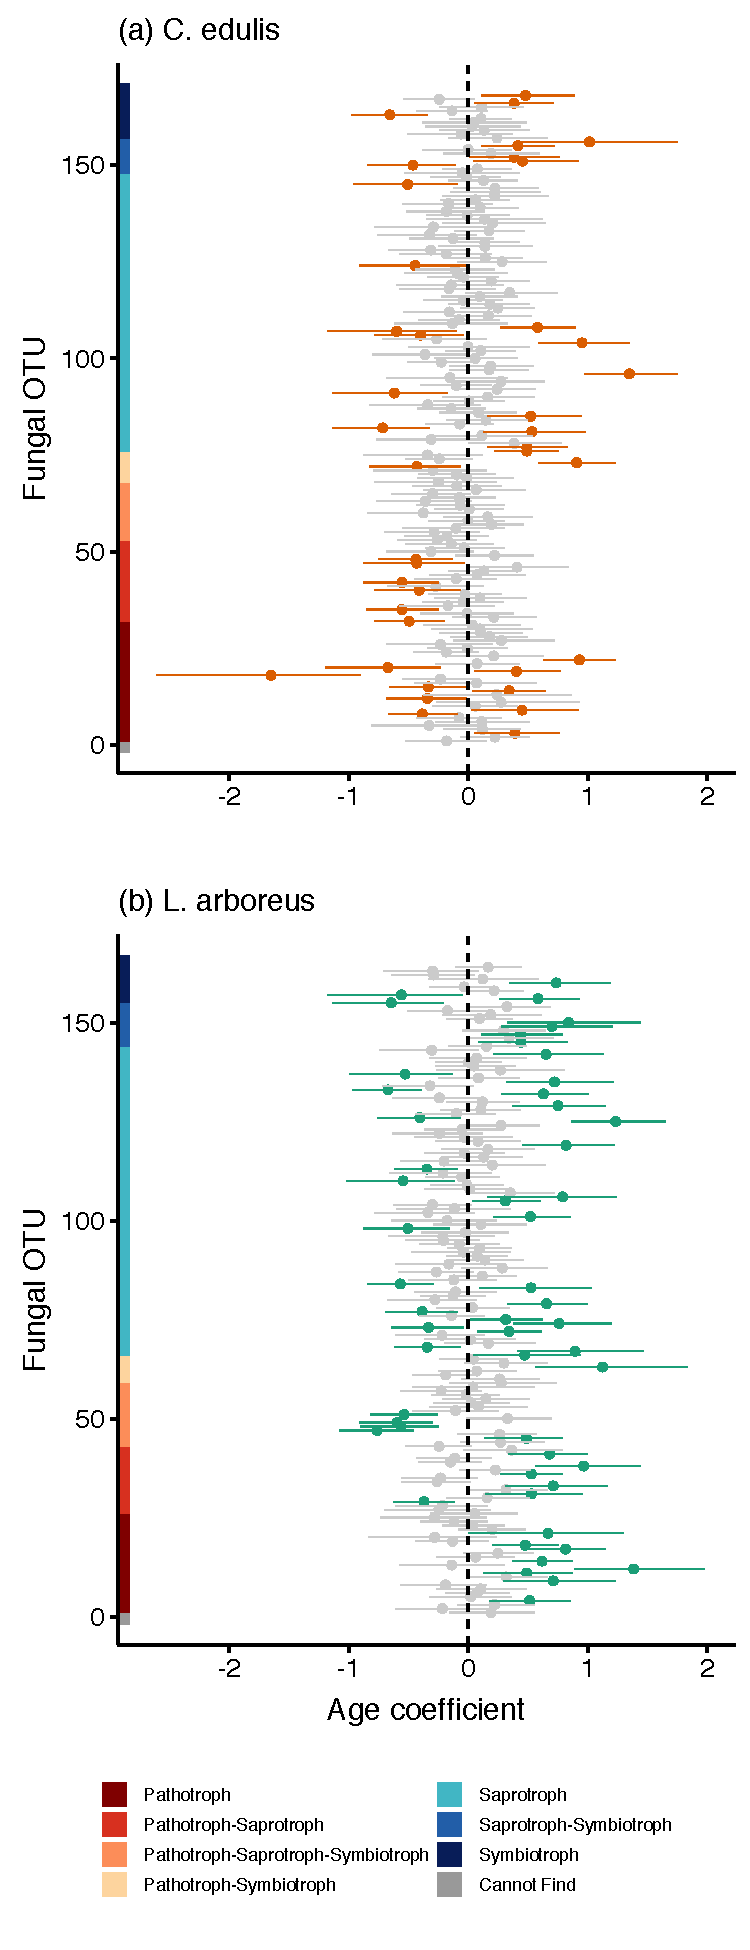
\includegraphics[width=7cm]{Chapter5/Funguild_HMSC_FungiSpecies_CombinedIndividual_Full2015Total_Long.pdf}}
	\caption[Predicted temporal trends and potential functional guilds of fungal OTUs associated with (a) \textit{C. edulis} and (b) \textit{L. arboreus}.]
	{\hspace{1mm} Predicted temporal trends and potential functional guilds of fungal OTUs associated with (a) \textit{C. edulis} and (b) \textit{L. arboreus}. Model fitting was performed for the two plant species separately. Points and line segments represent the mean and the 95$\%$ credible interval of the fitted age coefficient (x-axis) for different fungal OTUs (y-axis). Significant age coefficients are colored (orange for \textit{C. edulis}; green for \textit{L. arboreus}) and insignificant ones are in gray. Color codes along the y-axis are the predicted functional guild of the OTU obtained from \textit{FunGuild}.}
	\label{fig:Funguild_HMSC_Species_Individual_Full2015}
\end{figure}

